\section{集合的测量}
\label{sec:comb-set-measurement}
\label{sec:analysis-set-structures}

区间$[a,b]$的长度是$b-a$，但实轴上的集合未必是一个区间。
本节要解决的问题是：怎样把区间的长度推广到更一般的实数集合，并在原来的区间上仍得到$b-a$？
这样的长度概念将用于后面的积分：将输入范围分成若干块后，需要知道各块的大小，才能按这些大小累计函数取值。
有限集合的元素个数与加权计数提供另一类测量例子，可以先用它们说明为集合赋予大小时应遵守的相加规则。

距离与大小是两种不同的结构。同一个实轴及其通常距离，既可以测量区间长度，也可以计算集合中的点数；
因此，选定度量并没有唯一确定测度。

本节先用有限集合的计数与加权计数说明相加规则，再从区间长度构造Jordan测量，
并用有理点集说明有限覆盖的局限；随后引入可数集，用可数覆盖定义勒贝格外测度；
再通过精确分割条件选出可测集，在可测集上得到可数可加的勒贝格测度；
最后把这些性质抽象为一般测度空间，研究集合列的测度、零测集与集合的逼近。

\subsection{有限集与Jordan测量}
\label{sec:comb-counting-to-weight}

我们先把目标限制在有界的实数集合上，希望给这些集合建立与区间长度相容的测量方法。
例如$[0,1]\cup[2,3]$由两段互不重叠、长度各为$1$的区间组成，总长度应为$2$。
这说明所求的测量应满足一条规则：集合分成有限个两两不交的部分时，总量等于各部分测量值之和。

下面先在有限集合上用计数和加权计数说明这条规则，再回到实轴。
实轴上的长度将从区间出发，先计算有限个区间的并，再用这些简单集合逼近更一般的有界集合；
只有当内部与外部的长度估计能逼近同一个数时，才用这个数定义集合的Jordan测量。

\subsubsection{有限集的测量}

\paragraph{计数与加权计数}

在有限集合上，最直接的测量是数元素个数；若不同元素代表不同的份量，还可以给每个元素指定权重。
设$X=\{x_1,\ldots,x_m\}$中的点互异，每点带有非负权重$w_i$。
把落在$A\subseteq X$中的点的权重相加，定义
\[
 \mu(A)=\sum_{i:x_i\in A}w_i.
\]
所有$w_i=1$时，$\mu(A)=|A|$；改变权重时，元素不变，测量值却可以改变。
例如$X=\{a,b\}$，给$a,b$的权重分别为$1,2$，就有
$\mu(\{a\})=1$、$\mu(\{b\})=2$、$\mu(X)=3$。

若$A_1,\ldots,A_k$两两不交，每个点只落入其中一组，故
\[
 \mu\left(\bigcup_{j=1}^k A_j\right)=\sum_{j=1}^k\mu(A_j).
\]
这称为\term{有限可加性}（finite additivity）。它沿用计数的加法规则，
但相加的是各组的权重，不必是元素个数。

\paragraph{集合权重与函数值}

前面的$\mu(A)$只测量集合$A$本身。后面还要在集合上累计函数取值，届时每个点的贡献等于函数值乘以该点的权重。
例如固定前面的$X=\{a,b\}$，若$f(a)=3,f(b)=-1$，
不加权的取值和为$3-1=2$；按上述权重求和则为$3\cdot1+(-1)\cdot2=1$。
两种规则下的集合权重分别为$2$与$3$，函数的取值和则分别为$2$与$1$。
表~\ref{tab:analysis-metric-measure-integral}列出这些计算；后面的积分将把这种加权累计扩展到更一般的函数。
\begin{table}[htbp]
 \centering\small
 \begin{tabularx}{\linewidth}{@{}lXX@{}}
 \toprule
 考察对象 & 所用规则 & $X=\{a,b\}$上的结果\\
 \midrule
 元素个数 & 每点计$1$ & $|X|=2$\\
 集合权重 & $a,b$分别计$1,2$ & $\mu(X)=3$\\
 数值的等权累计 & 取值为$3,-1$ & $3-1=2$\\
 数值的加权累计 & 同一取值采用权重$1,2$ & $3-2=1$\\
 \bottomrule
 \end{tabularx}
 \caption{有限计数与加权累计。相同的元素范围和相同的数值取值仍可采用不同权重；只有先固定权重，累计值才有确定含义。}
 \label{tab:analysis-metric-measure-integral}
\end{table}

\paragraph{点数与长度}

有限集合的例子说明了不交部分如何相加，但每点计$1$的规则不能给出区间长度。
例如$[0,1]$和$[0,2]$都含有无限多个点，逐点计数都得到无穷，而它们的长度分别应为$1$和$2$。
所以，要推广区间长度，必须另行规定与几何长度相容的测量规则。

单点$[a,a]$的长度为$0$，有限个单点的并也应有长度$0$。这与非退化区间长度为正并不矛盾：区间不能写成有限个单点的并，有限可加性并不适用于将它拆成全部单点的操作。后面还会说明，非退化区间也不能按可数个单点列举。

我们下面以区间长度为起点，先给能由有限个区间组成的集合计算长度，再研究不能这样表示的集合。

\subsubsection{Jordan测量}

\paragraph{区间长度与初等集}

一个区间的长度由端点决定；有限个区间组成的集合，也可以先拆成互不重叠的小段再相加。

为反复使用这类可以直接计算长度的集合，先给它们一个名称。
对端点为$a\leq b$的有界区间$I$，规定长度为$\ell(I)=b-a$，不因端点是否包含而改变；
单点与空集的长度为$0$。

我们把有限个这样的区间的并称为\term{初等集}（elementary set），空集也约定为初等集。
例如$[0,1]\cup[2,3]$是初等集，可以将两段长度相加得到$2$。
区间发生重叠时，需要先消除重复计算：$[0,2]\cup[1,3]=[0,3]$的长度为$3$，不能把原来两段的长度直接相加为$4$。

一个初等集可以有多种区间表示。将所有端点排序后，按相邻端点间的开区间及端点本身切分，得到有限个两两不交的小段；只对属于该集合的小段长度求和，记为$\ell(B)$。
若采用另一种表示，把两组端点一起排序，便得到共同的细分；
区间从$c$处分成两段时，$(c-a)+(b-c)=b-a$，所以细分不改变总长度。
因此，$\ell(B)$不依赖原来的表示。

由同一细分可知，初等集的并、交、差仍为初等集；
不交初等集的长度有限可加。一般有限覆盖则只给出不等式：
若$B\subseteq\bigcup_{j=1}^k B_j$，有
$\ell(B)\leq\sum_{j=1}^k\ell(B_j)$，因为重叠小段可能在右侧被重复计算。

\paragraph{内容量与外容量}

初等集的长度已经可以计算，但有界集合只要求一个集合包含在某个有限区间内，并不要求它本身由有限个区间组成。
例如
\[
 E=\{1,1/2,1/3,\ldots\}\subseteq[0,1]
\]
就是一个有界集合，但它不是由有限个区间组成的初等集。

对任意$u>0$，$E\cap[u,1]$中的点$1/n$都满足$n\leq1/u$，所以这一部分只有有限多个点。
因此$E$不包含任何正长度区间：假如包含，就能从中截取一段左端点大于$0$的正长度区间，与刚才的有限性矛盾。若用有限个区间恰好拼出$E$，这些区间就只能退化成单点；有限个单点又不能组成$E$中的无限多个点。
所以前面针对初等集的长度公式尚不能直接用于$E$。

为了能对$E$这样的集合进行测量，一种办法是保留初等集作为计算工具，用包含关系给出长度估计。
把初等集$A$放在$E$内部，即$A\subseteq E$，$\ell(A)$就应是$E$长度的下界；
用初等集$B$包住$E$，即$E\subseteq B$，$\ell(B)$就应是上界。
我们希望内部估计尽可能大、外部估计尽可能小，因此分别取内部长度的上确界与外部长度的下确界。
这两个数未必相等；但如果相等的话，我们就可以用内部与外部的估计才共同确定一个长度值，以此来作为对$E$的测量。

我们下面将这两个界分别记下来，并以它们是否相等规定哪些有界集合可以用这种方法测量。
这里的候选都是有限区间并，所用的长度$\ell$已经在前面定义。
\begin{definition}[Jordan内容量与外容量]
\label{def:analysis-jordan-content}
对有界集合$E\subseteq\mathbb R$，定义\term{Jordan内容量}（Jordan inner content）与\term{Jordan外容量}（Jordan outer content）为
\[
 \begin{aligned}
 j_*(E)&=\sup\{\ell(A):A\subseteq E,\ A\text{为初等集}\},\\
 j^*(E)&=\inf\{\ell(B):E\subseteq B,\ B\text{为初等集}\}.
 \end{aligned}
\]
若$j_*(E)=j^*(E)$，称$E$为Jordan可测集，二者的共同值记为$j(E)$，称为它的\term{Jordan测量}（Jordan measure）值。
\end{definition}

有界性保证外部候选非空且长度有限；空集是内部候选，所以
$0\leq j_*(E)\leq j^*(E)<\infty$。
上下确界不要求由某个最佳初等集取得。
例如$E$本身是初等集时，内外都可选$E$，故$j(E)=\ell(E)$。
这保证新的定义保留了原来的区间长度与有限区间并的长度，有限点集的测量值也仍为$0$。

再看刚才的$E=\{1/n:n\geq1\}$。它不含正长度区间，内部初等集只能是有限点集，所以
\[
 j_*(E)=0
\]

对每个整数$N\geq2$，取
\[
 B_N=\{1,1/2,\ldots,1/(N-1)\}\cup[0,1/N].
\]
前$N-1$个点分别由单点覆盖，其余点全部落在$[0,1/N]$内，故$E\subseteq B_N$。
由于$B_N$是初等集，长度为$1/N$，所以$0\leq j^*(E)\leq1/N$对所有$N\geq2$成立，从而
\[
 j^*(E)=0
\]

内外容量相等，说明这个不属于初等集的无限点集仍然Jordan可测，而且$j(E)=0$。
这里的长度值来自有限逼近的误差$1/N$趋于零。

\paragraph{有限逼近与可加性}

内外数值相等也可以改写成误差条件：$E$为Jordan可测集，当且仅当对每个$\varepsilon>0$，
存在初等集$A\subseteq E\subseteq B$，使$\ell(B)-\ell(A)<\varepsilon$。
正向根据上确界和下确界各选一个误差小于$\varepsilon/2$的候选；
反向利用$j_*(E)$与$j^*(E)$始终夹在这两个长度之间。

这个夹逼条件还保证有限次集合运算保持Jordan可测性。
例如分别以$A_E\subseteq E\subseteq B_E$和$A_F\subseteq F\subseteq B_F$夹住两个集合，
它们的并可由$A_E\cup A_F$、$B_E\cup B_F$夹住，
新上下界之间的长度差不超过原来两份误差之和。
交集使用内、外逼近的交；差集使用$A_E\setminus B_F$与$B_E\setminus A_F$，
漏出的部分同样包含于原来的两份误差中。
因此，有限并、交、差均保持可测性。

若$E,F$还不交，内部逼近$A_E,A_F$也不交，于是
\[
 \ell(A_E)+\ell(A_F)
 \leq j_*(E\cup F)\leq j^*(E\cup F)
 \leq\ell(B_E)+\ell(B_F).
\]
让各份逼近误差趋零，得到$j(E\cup F)=j(E)+j(F)$。
这就是Jordan测量的有限可加性；它依赖有限次逼近误差仍能控制，而非任意多次并的封闭性。

\subsubsection{Jordan测量的局限}

\paragraph{有理点集的内外容量}

前面的倒数点集$E$虽然不是初等集，仍能用有限区间并把外部长度压到任意小。
这是否意味着每个有界集合都能这样处理？我们下面考察$Q_0=\mathbb Q\cap[0,1]$，说明Jordan方法使用的有限逼近并不能处理任意的有界集合。

先看$Q_0$在区间中的分布。任意非退化实区间$(a,b)$（$a<b$）都含有有理数和无理数。
先找有理数：取正整数$q>1/(b-a)$，相邻分数$p/q$与$(p+1)/q$的间距$1/q$小于区间长度。
令$p$为满足$p>aq$的最小整数，则$(p-1)/q\leq a<p/q$，于是$p/q\leq a+1/q<b$，即$p/q\in(a,b)$。

再找无理数：对区间内的有理数$r$，取正整数$k$使$\sqrt2/k<b-r$，则$r+\sqrt2/k$位于$(r,b)$内；
它若是有理数，$\sqrt2=k(r+\sqrt2/k-r)$也将是有理数，矛盾。
所以$Q_0$和它在$[0,1]$内的补集都与每一段正长度子区间相交。

内部逼近因此很小：任何正长度区间都含有无理数，不可能完全落在$Q_0$中。
包含于$Q_0$的初等集只能由有限个单点组成，长度为零，所以
\[ 
 j_*(Q_0)=0
\]

外部逼近却受到另一种限制。设初等集$B$包含$Q_0$，把组成$B$的有限个区间的端点补齐，得到闭包$\overline B$；
补上有限个点不改变长度，所以$\ell(\overline B)=\ell(B)$。
若$[0,1]$内某点不在$\overline B$，由于$\overline B$闭，这个点附近就有一小段完全避开$B$。
这段在$[0,1]$内的部分含有有理数，与$Q_0\subseteq B$矛盾。
因此$[0,1]\subseteq\overline B$，从而$\ell(B) = \ell(\overline B) \geq 1$。
又因为$[0,1]$本身就是一个外部候选，得到
\[
 j^*(Q_0)=1.
\]

内部逼近和外部逼近两种估计之间始终相差$1$，所以$Q_0$不Jordan可测。

\paragraph{有限覆盖的限制}

$Q_0$无法Jordan可测的问题不在于区间分得还不够多。无论选一百个还是一百万个区间，只要仍是有限个，它们的并就是初等集，上面的证明仍迫使任何覆盖$Q_0$的总长度至少为$1$。
这与倒数点集的情形不同：倒数点集可以把除有限点以外的全部点装进靠近零的一个短区间，
而有理点集在$[0,1]$的每一小段中都出现，不能用一个越来越短的区间收拢剩下的点。

要突破这个下界，需要扩大允许使用的覆盖，而不是继续增加某一次有限覆盖的区间数。
如果能将$Q_0$列为$q_1,q_2,\ldots$，就可以给每个点分别安排一个开区间，
并把长度依次限制为$\varepsilon/2,\varepsilon/4,\varepsilon/8,\ldots$。
每个点都会被覆盖，而总长度由几何级数控制在$\varepsilon$以内；$\varepsilon$又可以任意小。
这里需要一列区间同时覆盖全部点，任意一个有限前段本身都未必覆盖$Q_0$。
图~\ref{fig:measure-countable-cover}对比了两种覆盖规则；右侧的前四项只展示长度如何分配，并未单独完成对全部有理点的覆盖。

\begin{figure*}[htbp]
 \centering
 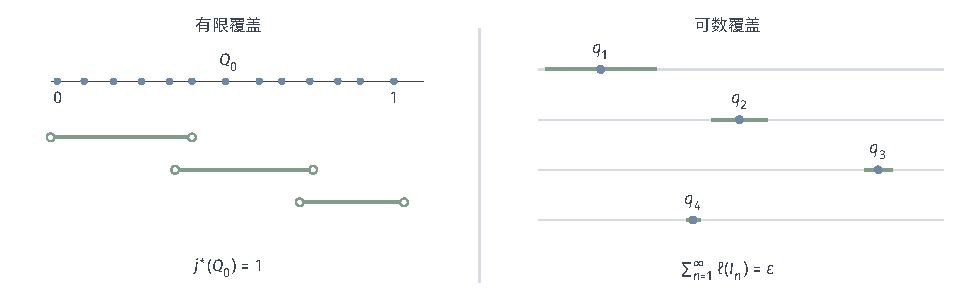
\includegraphics[width=169mm]{figures/01-mathematical-preliminaries-upper/01-mathematical-language-combinatorics-analysis-optimization/tikz/measure-countable-cover/figure.pdf}
 \caption{有限覆盖与可数覆盖。左侧画出一个有限开区间覆盖示例；对$Q_0=\mathbb Q\cap[0,1]$的任意有限区间覆盖，总长度均不小于$1$。右侧将一次完整覆盖改为可数个区间，图中取$\varepsilon=0.8$，只画列举中前四个点及其区间，长度依次为$\varepsilon2^{-n}$；使用全部区间时覆盖全部有理点，总长度为$\varepsilon$，并可随$\varepsilon$任意减小。点的有限示意不能表示有理点的完整稠密分布。}
 \label{fig:measure-countable-cover}
\end{figure*}


这给出新的思路：允许可数个区间组成一次完整覆盖，再用非负级数计算总长度。
第~\ref{sec:comb-countable-sets}节已经建立所需的列举与合并规则。下面先把这些规则用于覆盖，
再检查非负级数的合并，最后定义采用可数覆盖的外部长度估计。

\subsection{可数集与勒贝格外测度}
\label{sec:analysis-countable-outer-measure}

有限覆盖的限制已经给出了改变构造的理由：让每个可列举的点都能分到自己的小区间，
同时把所有区间的总长度控制住。可数覆盖使这两件事能够同时实现，因为区间有自然数编号，长度可以用已经学过的非负级数相加。

为使这一做法适用于后面的推导，先回用可数个可数集合的并仍可数，保证覆盖合并后仍在允许范围内；
非负双重级数可以合并，保证按组或统一编号计算覆盖长度得到同一个总和。
这些工具建立后，就能定义勒贝格外测度，并检查它既能改进有理点集的估计，又保留普通区间的长度。

\subsubsection{可数覆盖的编号与长度}

第~\ref{sec:comb-countable-sets}节已定义可数集，并用对角列举证明自然数对、有理数与可数个可数集的并可数。
因此$Q_0=\mathbb Q\cap[0,1]$可列为$\{q_1,q_2,\ldots\}$，每个点都能分到自己的小区间；
合并一列可数覆盖时，区间也仍可统一编号。
这里还需要检查总长度：改变非负项的列举方式，不能改变覆盖长度的总和。

\paragraph{非负双重级数的合并}

编号解决能否列举，级数规则还要保证改变列举方式不会改变覆盖总长度。
回用前面的非负项级数定义，对$a_n\in[0,\infty]$有
\begin{equation}
 \sum_{n=1}^{\infty}a_n
 =\sup_{N\geq1}\sum_{n=1}^Na_n\in[0,\infty].
 \label{eq:comb-nonnegative-sum-supremum}
\end{equation}
非负性使有限和随加入新项而增加，所以也可对所有有限索引集取上确界，结果相同。

对$a_{n,j}\geq0$，将双指标按任一无遗漏、无重复的顺序列成一个序列，总和便是
\[
 S=\sup_{F\subseteq\mathbb N_+^2,\,F\text{有限}}
          \sum_{(n,j)\in F}a_{n,j}.
\]
这个值等于$\sum_n\sum_j a_{n,j}$，也就是先对每一行求和、再把各行之和相加。下面分两个方向证明。

一个方向：任取有限索引集$F$，它只涉及有限多行，并在每一行中只取有限多项；
每行取出的部分不超过该行之和，所以$\sum_{(n,j)\in F}a_{n,j}\leq\sum_n\sum_ja_{n,j}$，对$F$取上确界得$S\leq\sum_n\sum_ja_{n,j}$。

反方向：固定行数$N$与任意$\varepsilon>0$，若各行之和都有限，对每个$n\leq N$选有限列数$J_n$，
使该行前$J_n$项之和超过整行之和减去$\varepsilon/N$。这些项组成一个有限索引集，所以
$S\geq\sum_{n=1}^N\sum_ja_{n,j}-\varepsilon$。令$\varepsilon\downarrow0$，再对$N$取上确界，得到$S\geq\sum_n\sum_ja_{n,j}$。
若某行之和为无穷，它的有限部分和可以超过任意给定的有限上界，同样迫使$S=+\infty$，两侧都为无穷。

证明只使用有限和与上确界的性质，这就为此处非负项的换序提供了依据，无须调用后文的积分换序定理。

\subsubsection{勒贝格外测度}
\label{sec:comb-length-and-lebesgue-measure}

\paragraph{可数区间覆盖}

前面已经证明$Q_0$可以列为$q_1,q_2,\ldots$，逐点安排小区间的方案因此可以实施。
我们把这种覆盖方式用于一般集合：对$E\subseteq\mathbb R$，选择有限或可数个有界开区间$I_j=(a_j,b_j)$，
只要求$E\subseteq\bigcup_j I_j$，称它们为$E$的可数区间覆盖。
区间可以重叠，也可以伸出$E$；它们的总长度为非负级数$\sum_j(b_j-a_j)$，允许等于$+\infty$。

“可数”限制的是覆盖区间的个数，不是$E$中的点数；一个开区间就可以覆盖含有不可数多个点的闭区间。
选择可数覆盖，是为了能逐项分配误差、用级数累计长度，并在合并覆盖时保留这两种能力。
前面没有给任意不可数族定义总长度，因此这里也不把“可数”直接换成不受限制的任意集合族。
采用开区间还使闭区间的有限子覆盖性质可以参与证明，下面将用它保证原来的区间长度不被改变。

\paragraph{勒贝格外测度的定义}

一次覆盖可能伸出集合，也可能重复覆盖某些位置，总长度只是一个外部估计，依赖于区间的选择。
为了尽量排除这些额外长度，我们对所有允许覆盖的总长度取下确界，得到勒贝格外测度。
\begin{definition}[勒贝格外测度]
\label{def:analysis-lebesgue-outer-measure}
对$E\subseteq\mathbb R$，定义其\term{勒贝格外测度}（Lebesgue outer measure）为
\begin{equation}
 m^*(E)=\inf\left\{\sum_{j=1}^{\infty}(b_j-a_j):
 \begin{array}{l}
 E\subseteq\bigcup_{j=1}^{\infty}(a_j,b_j),\\
 -\infty<a_j<b_j<\infty
 \end{array}\right\}.
 \label{eq:comb-lebesgue-outer-measure}
\end{equation}
这里也允许有限覆盖以及空集的空覆盖；空和为$0$。
\end{definition}

任意集合都能由覆盖整条实轴的一列区间覆盖，所以候选始终非空。
其下确界可为无穷，也不必由某个覆盖达到。
例如单点可以被任意短的开区间覆盖，其外测度为$0$；不存在长度为$0$的非空开区间来达到这个下确界。

\paragraph{空集与单调性}

空覆盖表明$m^*(\varnothing)=0$。
若$E\subseteq F$，任何覆盖$F$的区间族也覆盖$E$，
所以$E$的候选至少与$F$一样多，取下确界便得$m^*(E)\leq m^*(F)$。
这称为外测度的单调性，依据是允许覆盖之间的包含关系。

\paragraph{区间的外测度}

允许可数覆盖后，候选更多，下确界可能下降。我们希望有理点集的估计可以下降，同时必须检查普通区间的长度仍是原值。
先证明$m^*([a,b])=b-a$。上界用$(a-\varepsilon/2,b+\varepsilon/2)$覆盖$[a,b]$，再令$\varepsilon\downarrow0$。
下界必须控制每一种可数覆盖，不能只考察某一组区间。任取可数开区间覆盖，由闭区间的有限子覆盖性质，
其中有限个区间已经覆盖$[a,b]$，所以初等集的有限覆盖不等式给出
\[
 b-a\leq\sum_{j\in F}(b_j-a_j)\leq\sum_{j=1}^{\infty}(b_j-a_j),
\]
其中$F$是选出的有限索引集。对所有可数覆盖取下确界，得到反向界。
因此闭区间外测度等于长度；对任意端点型式的非退化区间$I$，
在它内部放入长度趋向$b-a$的闭区间，再用单调性夹逼，也得到$m^*(I)=b-a$。
无界区间包含任意长的有界闭区间，故其外测度为$+\infty$。

\paragraph{可数点集的外测度}

现在回到推动构造的例子，检验可数覆盖是否真正突破了有限覆盖的限制。
设$E=\{x_1,x_2,\ldots\}$可数，任给$\varepsilon>0$，对每个$n$取
\[
 I_n=\bigl(x_n-\varepsilon2^{-n-1},\ x_n+\varepsilon2^{-n-1}\bigr).
\]
每个点$x_n$都落入$I_n$，所以这列区间覆盖全部$E$，且$\ell(I_n)=\varepsilon2^{-n}$。
这组覆盖满足
\[
 0\leq m^*(E)\leq\sum_{n=1}^{\infty}\varepsilon2^{-n}=\varepsilon.
\]
由于$\varepsilon$任意，得到$m^*(E)=0$，有限集也可同样处理。
这里每个覆盖区间的长度都为正；趋向零的是全部覆盖的总长度上界，而不是在相加一些未定义的正“无穷小”。

特别地，$m^*(Q_0)=0$，尽管它的Jordan外容量为$1$。
有限覆盖的下界为$1$，可数覆盖却能把总长度压到任意给定的正误差以内；改变的是一次完整覆盖所允许的区间族。
这与$m^*([0,1])=1$也不矛盾：$Q_0$可数，能够逐点编号，整个区间却不可数，无法给其中全部点各分配上述自然数编号。

到这里，我们已经得到每个集合的外测度值，还没有证明这些值在不交集合之间能够精确相加。
因此$m^*(Q_0)=0$先回答了外部估计的问题；要把外测度用于稳定的分块累计，还需要下面的可加性与可测性。

\subsubsection{可数可加性}

\paragraph{可数可加性的要求}

新的覆盖方式已经处理了可数次累计，我们也希望测量规则能处理可数次不交分割。
例如，若一个可数点集能作为各个单点的不交并参与精确相加，它的总长度就应由单点长度之和确定。

一般地，对赋值$\nu$，希望有
\[
 \nu\left(\bigcup_{n=1}^{\infty}E_n\right)=\sum_{n=1}^{\infty}\nu(E_n),
 \qquad E_i\cap E_j=\varnothing\ (i\neq j),
\]
其中并集与各部分都应在$\nu$的赋值范围内。
这称为\term{可数可加性}（countable additivity），右侧是已经定义的非负项级数。

区间不可数，因而此要求不允许把一个区间拆成全部单点后当作可数级数求和；
单点外测度为零与区间外测度为正并不矛盾。

\paragraph{外测度的可数次可加性}

先从已经建立的覆盖构造推出一个能够保证的结论：把每个集合的覆盖合并，就得到并集的覆盖，
所以并集的外测度不超过各部分外测度之和。这只是不等式，并且不要求各集合不交。
这项性质称为\term{可数次可加性}（countable subadditivity）；名称中的“次”表示这里保证的是上界，不是精确相等。

每个集合未必有达到外测度的最优覆盖，证明时只能选近似最优覆盖。
因此需要把第$n$组的误差限制为$\varepsilon2^{-n}$，使合并无穷多组后总误差仍不超过$\varepsilon$。
\begin{theorem}[勒贝格外测度的可数次可加性]
\label{thm:analysis-outer-subadditivity}
对任意$E_1,E_2,\ldots\subseteq\mathbb R$，有
\begin{equation}
 m^*\left(\bigcup_{n=1}^{\infty}E_n\right)
 \leq\sum_{n=1}^{\infty}m^*(E_n).
 \label{eq:analysis-outer-subadditivity}
\end{equation}
\end{theorem}
\begin{proof}
若右侧为$+\infty$，不等式直接成立。
设右侧有限，则每个$m^*(E_n)$有限。给定$\varepsilon>0$，由下确界定义，
为每个$E_n$选择覆盖$\{I_{n,j}:j\geq1\}$，使
\[
 E_n\subseteq\bigcup_j I_{n,j},\qquad
 \sum_j\ell(I_{n,j})<m^*(E_n)+\varepsilon2^{-n}.
\]
空集可以取空覆盖，有限覆盖直接作为有限组处理。
所有$I_{n,j}$覆盖$\bigcup_nE_n$；可数个可数集的并仍可数，故它们是允许使用的一组覆盖。
再由非负双重级数的合并规则，
\[
 \begin{aligned}
 m^*\left(\bigcup_nE_n\right)
 &\leq\sum_{n,j}\ell(I_{n,j})\\
 &=\sum_n\sum_j\ell(I_{n,j})
 \leq\sum_nm^*(E_n)+\varepsilon.
 \end{aligned}
\]
最后让$\varepsilon\downarrow0$，得到所需不等式。
\end{proof}

\paragraph{一般外测度}

刚才的证明只给出不等式，尚未要求不交集合的值精确相加。
把已经得到的三条性质抽取出来，便得到可用于其他测量构造的一般概念。
\begin{definition}[外测度]
\label{def:analysis-outer-measure}
集合$X$上的映射$\mu^*:\mathcal P(X)\to[0,\infty]$，若满足
\[
 \begin{gathered}
 \mu^*(\varnothing)=0,\\
 A\subseteq B\Longrightarrow\mu^*(A)\leq\mu^*(B),\\
 \mu^*\left(\bigcup_{n=1}^{\infty}E_n\right)\leq\sum_{n=1}^{\infty}\mu^*(E_n)
 \quad(E_n\subseteq X),
 \end{gathered}
\]
则称为\term{外测度}（outer measure）。
\end{definition}
勒贝格外测度是一个实例。刚才的覆盖合并证明了定义中的第三条性质，却没有给出反向不等式。
即使$E_n$两两不交，分别覆盖它们的开区间也可能彼此重叠；集合不交并不会自动使覆盖的长度精确相加。
反过来，把覆盖并集的区间按任意集合切开，所得部分又未必是区间，不能直接沿用区间长度公式来分配总量。
因此，不能仅凭这三个条件便把式~\eqref{eq:analysis-outer-subadditivity}中的不等号改为等号。

下一步要补上的，是集合与这套外部估计之间的分割相容性：用一个集合切分任意测试集，切分后两部分的外测度之和仍等于原值。
我们将把满足这个要求的集合选出来，再证明在它们组成的范围内，不交可数并确实能够精确相加。

\subsection{可测集与勒贝格测度}
\label{sec:analysis-lebesgue-measurable-construction}

现在有两个不同的问题：一个集合能否取得外测度值，以及它能否在分割计算中保持精确相加。
第一个问题已经解决，任意集合都有$m^*$值；第二个问题还没有由覆盖构造保证。
要为积分准备可以反复分块的测量规则，就需要找出能够保持精确分割的集合，这就是引入可测集的原因。

下面保留原来的$m^*$数值，要求一个集合用来切分任何测试集时，都不改变分割前后的总量。
我们先写出这个条件，再证明满足条件的集合对取补和可数并封闭，最后证明限制到这一范围的$m^*$具有可数可加性。

\subsubsection{可测性的要求}

\paragraph{精确分割}

固定一个待检验的集合$A$，再任取测试集$E$。$A$把$E$分成落在$A$内的部分和落在$A$外的部分：
\[
 E=(E\cap A)\cup(E\setminus A),\qquad
 (E\cap A)\cap(E\setminus A)=\varnothing.
\]
次可加性已经保证$m^*(E)\leq m^*(E\cap A)+m^*(E\setminus A)$。
若要分割不改变总量，还需反向不等式；缺少它时，两部分分别作外部估计，所得总和可能比整体的外部估计大。

先用一个有限例子说明，外测度的三个公理确实没有自动排除这种情况。
在两点集合$X=\{a,b\}$上，令$\mu^*(\varnothing)=0$，每个非空子集的值都为$1$。
它单调，而且只要一列集合的并非空，右侧就至少有一项为$1$，所以满足可数次可加性。
但取$E=X$、$A=\{a\}$时，
\[
 1=\mu^*(X)<\mu^*(\{a\})+\mu^*(\{b\})=2.
\]

这是一般外测度的例子，用来说明仅有三个公理不足以推出精确相加，并不是勒贝格外测度的不可测集构造。
图~\ref{fig:measure-exact-splitting}把这个反例与区间的精确分割放在一起，展示可测性条件要排除的总量变化。

\begin{figure*}[htbp]
 \centering
 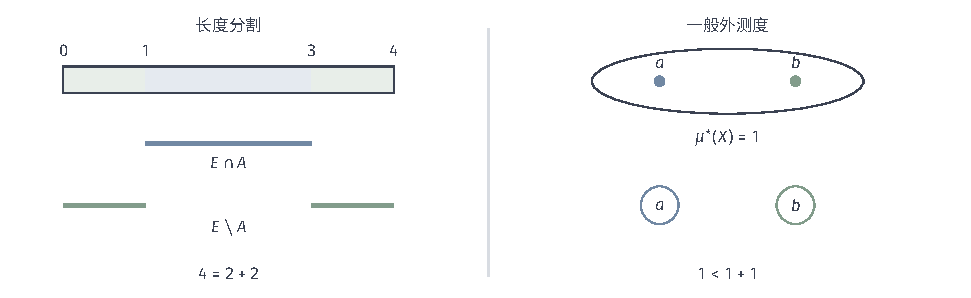
\includegraphics[width=169mm]{figures/01-mathematical-preliminaries-upper/01-mathematical-language-combinatorics-analysis-optimization/tikz/measure-exact-splitting/figure.pdf}
 \caption{精确分割与一般外测度的差别。左侧用$A=[1,3]$分割测试集$E=[0,4]$，落在$A$内的长度为$2$，外部两段总长度也为$2$，两者恢复原来的$4$；有限端点不改变长度。右侧使用正文两点空间的外测度，整体值为$1$，拆成两个单点后的值之和为$2$。右侧并非勒贝格不可测集的图像；左侧也只画了一个测试集，可测性定义要求对每个测试集都有精确等式。}
 \label{fig:measure-exact-splitting}
\end{figure*}

勒贝格外测度也存在不能保持精确分割的集合；这类不可测集的存在与构造可参考测度论教材\scite{math-hunter2011measure,math-folland1999real}，这里不展开。
下面直接以精确分割为条件选取可测集，并证明这类集合上的可加性。

\paragraph{可测集的定义}

我们希望$A$能够在不同范围的计算中反复参与分割，因此条件不能只针对某个预先选好的$E$。
下面要求等式对所有测试集成立，并把满足要求的$A$称为勒贝格可测集。
\begin{definition}[勒贝格可测集]
\label{def:analysis-lebesgue-measurable-set}
集合$A\subseteq\mathbb R$称为\term{勒贝格可测集}（Lebesgue measurable set），若对每个$E\subseteq\mathbb R$都有
\begin{equation}
 m^*(E)=m^*(E\cap A)+m^*(E\setminus A).
 \label{eq:comb-caratheodory-measurability}
\end{equation}
全体勒贝格可测集组成的集合族记为$\mathcal L(\mathbb R)$。
\end{definition}

这称为Carathéodory可测性条件。
由于其中一个不等式已经成立，验证可测性只需证明
$m^*(E)\geq m^*(E\cap A)+m^*(E\setminus A)$。
必须检验每个$E$，因为只令$E=A$会得到对任意集合都成立的恒等式，无法区分哪些分割与外测度相容。
“可测”并不表示此前无法给$A$求值；$m^*(A)$对任意$A$都已定义。新增要求是$A$与所有测试集的分割相容。

外测度为零的集合不需要逐个寻找特殊分割。下面先证明一个通用结论，以后处理零测余量和完备性时都可使用。
\begin{lemma}[零外测度集的子集可测]
\label{lem:analysis-zero-outer-measure-measurable}
若$N\subseteq\mathbb R$且$m^*(N)=0$，则每个$D\subseteq N$都勒贝格可测，并且$m^*(D)=0$。
\end{lemma}
\begin{proof}
单调性先给出$m^*(D)=0$。对任意测试集$E$，有
\[
 m^*(E\cap D)+m^*(E\setminus D)=0+m^*(E\setminus D)\leq m^*(E).
\]
结合外测度次可加性给出的反向不等式，得到可测性所需的精确分割等式。
\end{proof}
前面已证明$m^*(Q_0)=0$，所以此引理立即说明$Q_0$勒贝格可测。

后面把外测度限制到可测集上定义勒贝格测度时，$Q_0$的值仍为$0$。
取$E=[0,1]$还得到$m^*([0,1]\setminus Q_0)=1$：有理点与无理点都分布在每一小段中，却不因此占有相同的长度。
可测性由上述分割等式判断，而不是由集合看起来是否稠密、光滑或规则判断。

\subsubsection{可测集族}

前面的定义逐个检验一个集合能否精确切分任意测试集。接下来还要检验：这些可测集合经过取补、合并等运算后，是否仍然可测？

如果每次分块或合并都可能离开允许测量的范围，就无法反复使用这套测量方法。例如，每个单点$\{q_n\}$都Jordan可测，它们的可数并$Q_0$却不Jordan可测。
这说明允许每个部分参与测量，还不够保证合并后的对象也能参与测量。

勒贝格构造需要解决这个范围问题：先证明可测集族对所需运算封闭，再讨论合并后数值怎样相加。

\paragraph{取补与有限并}

取补对应保留分割的另一侧，有限并对应把有限块合为一块；先检查这两类操作，便能处理有限次分块计算。
下面始终以任意测试集$E$检验所得集合，沿用已经证明的次可加性作为其中一个方向。

空集满足$m^*(E)=0+m^*(E)$，所以可测。
把$A$换成$\mathbb R\setminus A$只交换式~\eqref{eq:comb-caratheodory-measurability}右边的两项，因此取补保持可测，特别地$\mathbb R$也可测。

若$A,B$可测，先用$A$分割$E$，再用$B$分割$E\setminus A$，得到
\[
 \begin{aligned}
 m^*(E)&=m^*(E\cap A)+m^*((E\setminus A)\cap B)\\
 &\quad +m^*(E\setminus(A\cup B))\\
 &\geq m^*(E\cap(A\cup B))+m^*(E\setminus(A\cup B)).
 \end{aligned}
\]
前两部分恰好组成$E\cap(A\cup B)$；次可加性使它们的外测度之和不小于这个并的外测度，得到所需反向不等式。
结合已有的次可加界，对每个$E$都有精确分割，所以$A\cup B$可测。
再由$A\cap B=(A^c\cup B^c)^c$和$A\setminus B=A\cap B^c$，得到有限交与差的可测性，这里的补集均相对于$\mathbb R$。
若$A,B$不交，以$A$分割$E\cap(A\cup B)$还给出
\[
 m^*(E\cap(A\cup B))=m^*(E\cap A)+m^*(E\cap B).
\]
反复应用可处理任意有限个不交可测集合。
这里同时得到了两件事：有限并仍在可测范围内；对不交的有限部分，切分前后的外测度精确相加。
后面处理可数并时，将先使用这两条有限结论，不预先假定无限情形已经成立。

\paragraph{可数并}

有限次合并已经不会离开可测范围，但一列集合的并未必能在有限步结束，仍需单独证明可数并的可测性。
证明的办法是先精确切出前$N$块，再让非负部分和随$N$增加，而不是直接调用尚未建立的测度可数可加性。
设$C_n$两两不交且可测，令$U_N=\bigcup_{n=1}^NC_n$、$U=\bigcup_{n=1}^{\infty}C_n$。
有限分割与外测度单调性给出，对每个$E$和每个$N$，
\[
 \begin{aligned}
 m^*(E)
 &=\sum_{n=1}^Nm^*(E\cap C_n)+m^*(E\setminus U_N)\\
 &\geq\sum_{n=1}^Nm^*(E\cap C_n)+m^*(E\setminus U).
 \end{aligned}
\]
因为$E\setminus U\subseteq E\setminus U_N$，上式对每个$N$都成立。
对非负部分和取上确界，便得到整列分割所需的下界；再用外测度的可数次可加性合并$E\cap C_n$，得到
\[
 m^*(E)\geq\sum_{n=1}^{\infty}m^*(E\cap C_n)+m^*(E\setminus U)
 \geq m^*(E\cap U)+m^*(E\setminus U).
\]
这就是$U$的可测性条件，故不交可测集的可数并可测。
若$A_n$不一定不交，令$C_1=A_1$、$C_n=A_n\setminus\bigcup_{j<n}A_j$。
每个$C_n$只用有限并与差集构成，所以已知可测；逐项去掉此前出现的部分，又使它们两两不交且并集不变。
对$C_n$应用刚才的结论，就证明了一般可数并仍可测。
至此，取补、有限并和可数并的运算都不会使我们离开$\mathcal L(\mathbb R)$。

\paragraph{$\sigma$代数}

刚才证明的封闭性质，正是后续反复分块和合并时需要的范围保证。
为了在其他对象集合上也使用同样的保证，下面把“包含全集、取补封闭、可数并封闭”统一定义为$\sigma$代数。
\begin{definition}[$\sigma$代数]
\label{def:analysis-sigma-algebra}
设$X$为集合。若子集族$\mathcal A\subseteq\mathcal P(X)$满足
\[
 \begin{gathered}
 X\in\mathcal A,\\
 A\in\mathcal A\Longrightarrow X\setminus A\in\mathcal A,\\
 A_1,A_2,\ldots\in\mathcal A
 \Longrightarrow\bigcup_{n=1}^{\infty}A_n\in\mathcal A,
 \end{gathered}
\]
则称$\mathcal A$为$X$上的\term{$\sigma$代数}（sigma-algebra）。
\end{definition}

由取补可得$\varnothing\in\mathcal A$；在有限集合族之后补空集，便得到有限并。
De Morgan公式又给出可数交：$\bigcap_nA_n=X\setminus\bigcup_n(X\setminus A_n)$。
可数交的封闭性也很实用：例如$\{a\}=\bigcap_{n\geq1}(a-1/n,a+1/n)$，一个点可以由一列邻域的交得到。
因此，只保证有限运算封闭还不能覆盖后面涉及无限过程的集合构造，$\sigma$代数将这些可数运算纳入同一个范围。

在当前的勒贝格构造中，$\mathcal L(\mathbb R)$先由精确分割条件选出，再由前面的推导证明它是$\sigma$代数；
没有先假定所有可测集合自动具有这些封闭性。
在抽象测量问题中，则可以先指定一个$\sigma$代数来规定允许测量的范围。
两种做法的起点不同，但得到的范围结构相同。

$\sigma$代数记录允许测量的子集，并保证这些子集经过所需的集合运算后仍在这一范围内；它没有给集合赋予大小，也没有单独保证任何数值的可加性。
所以接下来还要把已经构造的外测度放到这个可测范围上，证明它确实满足精确相加的规则。

\subsubsection{勒贝格测度}

\paragraph{限制外测度}

现在有了两个对象：$m^*$负责给集合赋值，$\mathcal L(\mathbb R)$负责保证取补和可数合并后仍在可测范围内。
我们保留$m^*$在可测集上的原值，把允许的输入从所有子集收缩为$\mathcal L(\mathbb R)$，并给这个限制后的赋值命名。
\begin{definition}[勒贝格测度]
\label{def:analysis-lebesgue-measure}
勒贝格外测度在$\mathcal L(\mathbb R)$上的限制
\[
 m:\mathcal L(\mathbb R)\to[0,\infty],\qquad m(A)=m^*(A),
\]
称为\term{勒贝格测度}（Lebesgue measure）。
\end{definition}

这一步没有重新计算任何可测集的大小：例如$m(Q_0)=m^*(Q_0)=0$，空集仍有$m(\varnothing)=0$。
改变的是赋值的定义域，而“它是测度”还需要下面的可数可加性证明。

\paragraph{不交可测并的可数可加性}

$\sigma$代数已经保证可数并是允许输入，因此等式左侧有定义；精确分割条件则使每个有限不交部分和都成为并集测量值的下界。
对这些下界取上确界，再结合外测度原有的次可加上界，就能把不等式收紧为等式。
\begin{theorem}[勒贝格测度的可数可加性]
\label{thm:analysis-lebesgue-countable-additivity}
若$A_n\in\mathcal L(\mathbb R)$两两不交，则
\[
 m\left(\bigcup_{n=1}^{\infty}A_n\right)=\sum_{n=1}^{\infty}m(A_n).
\]
\end{theorem}
\begin{proof}
记$A=\bigcup_n A_n$。前面已证明$A$可测；对每个$N$，由单调性与有限分割，
\[
 m(A)\geq m\left(\bigcup_{n=1}^NA_n\right)=\sum_{n=1}^Nm(A_n).
\]
对$N$取上确界，得到$m(A)\geq\sum_n m(A_n)$。
反向不等式正是外测度的可数次可加性，因为$m$与$m^*$在这些集合上相同。
\end{proof}

因此，可数并封闭与可数可加解决的是两个相接的问题：前者保证合并后的集合仍可测量，后者保证它的测量值等于不交部分之和。
从$m^*$到$m$也经过了两步：先由精确分割条件得到$\mathcal L(\mathbb R)$及其封闭性，再证明保留在这一范围上的数值具有可数可加性。
这两步共同使勒贝格测度能够用于反复的分块累计。
类似构造也适用于一般外测度；这里已经把一维长度所需的关键封闭性与可加性步骤给出，
更一般的表述可参考测度论教材\scite{math-hunter2011measure,math-folland1999real}。

\paragraph{区间与常见可测集}

可数可加性定理只适用于已经可测的集合，所以还要确认普通区间、开集等常用对象确实属于$\mathcal L(\mathbb R)$。
先从半直线开始：它只需在一个位置切分区间，容易将可测性条件还原为已知长度之和。

固定$t\in\mathbb R$，考虑半直线$H=(-\infty,t]$。
若$m^*(E)<\infty$，给定$\varepsilon>0$，选择总长度小于$m^*(E)+\varepsilon$的开区间覆盖$\{I_j\}$。
将每个$I_j$在$t$处切成两段；两段可能是开区间、半开区间或空集，
其外测度已知等于各自长度，而两段长度之和仍是$\ell(I_j)$。
分别覆盖$E\cap H$和$E\setminus H$，由外测度的次可加性得
\[
 \begin{aligned}
 &m^*(E\cap H)+m^*(E\setminus H)\\
 &\quad\leq\sum_j\bigl[m^*(I_j\cap H)+m^*(I_j\setminus H)\bigr]\\
 &\quad=\sum_j\ell(I_j)<m^*(E)+\varepsilon.
 \end{aligned}
\]
令$\varepsilon\downarrow0$就得到所需反向不等式。
若$m^*(E)=\infty$，次可加性已迫使分割后总和也为无穷，等式自动成立。
所以$H$可测。

半直线的差给出半开区间；可数并与交又给出其他端点型式的区间和单点。
任意开集是其中所有有理端点开区间的并：对每个点先取完全落在开集内的小区间，再利用有理数的稠密性缩小端点。
有理端点对可数，故这是一组可数并，所以开集、其补集及后续可数集合运算所得的集合都可测。
区间长度结论也随之保留为
\[
 m((a,b))=m([a,b])=m([a,b))=b-a,\qquad m(\{a\})=0.
\]

\paragraph{Borel集合}

区间与开集已经可测，但以后往往从它们出发反复取补、作可数并或可数交。
为了统一指明这些操作必然产生的集合，下面定义包含全部开区间的最小$\sigma$代数。

这样的最小范围确实存在：$\mathcal P(\mathbb R)$是一个包含所有开区间的$\sigma$代数，故候选不空。
把全部候选取交，所得集合族仍包含全集，并且取补、可数并后仍属于每个候选，所以交族本身也是$\sigma$代数。
它包含所有开区间，又包含于每个候选，因而正是所需的最小范围，称为由开区间生成的$\sigma$代数。
\begin{definition}[Borel $\sigma$代数]
\label{def:analysis-borel-sigma-algebra}
实轴上由所有开区间$(a,b)$（$a<b$）生成的最小$\sigma$代数记为$\mathcal B(\mathbb R)$，称为\term{Borel $\sigma$代数}（Borel sigma-algebra）。
对$X\subseteq\mathbb R$，令
\[
 \mathcal B(X)=\{X\cap B:B\in\mathcal B(\mathbb R)\},
\]
称为$X$上的Borel $\sigma$代数；其中的集合称为Borel集合。
\end{definition}

前面对开集的表示说明，这也等于所有开集生成的$\sigma$代数。
例如$\{a\}=\bigcap_{n\geq1}(a-1/n,a+1/n)$是Borel集合，可数点集因而也是Borel集合。
各范围之间有
\[
 \mathcal B(\mathbb R)\subseteq\mathcal L(\mathbb R)\subseteq\mathcal P(\mathbb R),
 \qquad m=m^*\big|_{\mathcal L(\mathbb R)}.
\]
第一个包含关系来自可测范围的封闭性：$\mathcal L(\mathbb R)$已经是包含所有开区间的$\sigma$代数，必包含最小的$\mathcal B(\mathbb R)$。
第二个包含关系只说明可测集也是实轴子集；它不表示全部子集都可测。
这里$\mathcal B(\mathbb R)$与$\mathcal L(\mathbb R)$都是集合族，规定允许的范围；$m$与$m^*$是给集合赋值的函数，职责不同。
勒贝格可测范围仍不是所有子集；不可测集的构造不在这里展开。

\paragraph{Jordan测量与勒贝格测度}

前面已经说明区间长度保持不变，现在进一步检验每个Jordan可测集是否都被新构造保留，且测量值相同。
证明中的零测余量由引理~\ref{lem:analysis-zero-outer-measure-measurable}处理：外测度为零的集合的任意子集都已可测，因此内部Borel部分之外的零测误差不会破坏可测性。

若$E$为Jordan可测集，对每个$n$取初等集$A_n\subseteq E\subseteq B_n$，
使$\ell(B_n)-\ell(A_n)<2^{-n}$。
令$A=\bigcup_nA_n$、$B=\bigcap_nB_n$，则$A,B$均为Borel集合，且$A\subseteq E\subseteq B$。
由于$B\setminus A\subseteq B_n\setminus A_n$，有
$m(B\setminus A)\leq\ell(B_n)-\ell(A_n)<2^{-n}$对所有$n$成立，故$m(B\setminus A)=0$。
该引理表明$E\setminus A$可测，于是$E=A\cup(E\setminus A)$也可测。
再由$j_*(E)\leq m(E)\leq j^*(E)$得到$m(E)=j(E)$。

因此Jordan可测集都勒贝格可测，数值保持一致；$Q_0$则说明逆向不成立。
它虽然在每个小区间中都稠密，却是可数Borel集合，勒贝格测度为零。
可测性的边界由分割性质规定，不由“看起来复杂”来判定。

\subsection{测度空间与测度的性质}
\label{sec:comb-measurable-sets-and-weights}

勒贝格长度已经形成一套完整的测量设定：实轴$\mathbb R$给出对象范围，$\mathcal L(\mathbb R)$给出允许测量的子集族，$m$给这些子集赋值。
有限加权计数也具有相同的三层结构，只是对象范围和具体赋值不同。

为了把后面的推导同时用于长度、计数与其他权重，现在把三层结构分别抽象出来。
先记录对象范围和可测集合族，得到可测空间；再要求赋值满足空集为零与可数可加性，得到测度；
将三项放在一起才得到测度空间。之后有关集合列与零测例外的结论，就可以从共同条件推出，不必对每一种测量重新证明。

这里改变的是讨论范围：此前通过区间覆盖构造了一个特定的函数$m$，现在将它已满足的性质提炼为一般赋值的共同要求。
勒贝格测度本身的定义和值都不改变；它成为一般测度的一个实例，计数和其他权重也能纳入同一套结论。
一般测度不必从实轴区间覆盖出发构造，也不必把区间赋值为长度。
图~\ref{fig:measure-abstraction}将这条具体构造与抽象过程分开，并对照三项结构。

\begin{figure*}[htbp]
 \centering
 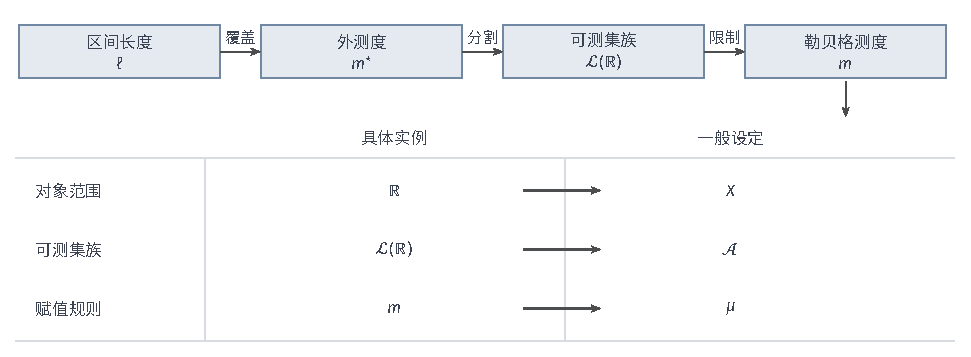
\includegraphics[width=169mm]{figures/01-mathematical-preliminaries-upper/01-mathematical-language-combinatorics-analysis-optimization/tikz/measure-abstraction/figure.pdf}
 \caption{从勒贝格测度到一般测度。上部是前文在实轴上完成的具体构造：区间长度经可数覆盖得到外测度，再用精确分割选出可测集，将外测度限制到这一集合族上得到$m$。中部将对象范围、允许集合族与赋值规则对应为$X$、$\mathcal A$、$\mu$，其中$\mathcal A$为$X$上的$\sigma$代数，$\mu:\mathcal A\to[0,\infty]$。测度$\mu$须满足空集为零和两两不交可测集合的可数可加性。前两项组成可测空间$(X,\mathcal A)$，三项共同组成测度空间$(X,\mathcal A,\mu)$。在同一$(\mathbb R,\mathcal L(\mathbb R))$上，勒贝格测度$m$给单点赋值$0$，计数测度$\nu$则赋值$1$，说明允许测量的集合相同，赋值仍可不同。因此勒贝格测度是一种具体测度，一般测度的定义不限定为长度，也不要求都按上部的区间覆盖步骤构造。}
 \label{fig:measure-abstraction}
\end{figure*}


\subsubsection{测度空间}

\paragraph{可测空间}

只给出集合$X$，还没有指定哪些子集可以参与测量；允许范围需要单独记录，并应对取补和可数并封闭。
因此，下面把$X$与它上面选定的$\sigma$代数组合起来，暂不指定任何测量值。

\begin{definition}[可测空间]
设$\mathcal A$为$X$上的$\sigma$代数，二元组$(X,\mathcal A)$称为\term{可测空间}（measurable space）。
$\mathcal A$中的集合称为相对于$\mathcal A$的\term{可测集合}（measurable set）。
\end{definition}
例如$X=\{a,b,c\}$上的
$\mathcal A=\{\varnothing,\{a,b\},\{c\},X\}$是一个$\sigma$代数。
这个例子把$a,b$作为不能单独分开的同一块，而$c$单独成块；列出的集合就是这些块的各种并。
取补会选出剩余块，可数并也仍是这些块的并，所以$\mathcal A$确实是$\sigma$代数。
在这个可测空间中，$\{a,b\}$属于允许范围，$\{a\}$却不属于它。
这只表示当前没有把$\{a\}$列为可测对象，并不表示它在任何测量设定下都不能测量；改选$\mathcal P(X)$就会允许全部子集。

所以，抽象可测空间中的“可测”是相对于指定的$\mathcal A$而言的。
前面的“勒贝格可测”则指通过$m^*$的精确分割条件得到的特定范围$\mathcal L(\mathbb R)$；它为一般定义提供了一个已经证明满足要求的实例。

\paragraph{测度}

可测空间保证集合运算后的对象仍在允许范围内，却还没有给任何集合规定数值。
下面借鉴已经证明的勒贝格可数可加性，对一般赋值提出同样要求；右侧仍用非负级数求和，允许值为$+\infty$。
\begin{definition}[测度]
设$(X,\mathcal A)$为可测空间。映射$\mu:\mathcal A\to[0,\infty]$若满足$\mu(\varnothing)=0$，并且对任意两两不交的$A_1,A_2,\ldots\in\mathcal A$有
\begin{equation}
 \mu\left(\bigcup_{n=1}^{\infty}A_n\right)
   =\sum_{n=1}^{\infty}\mu(A_n),
 \label{eq:comb-countable-additivity}
\end{equation}
则称$\mu$为\term{测度}（measure），这个等式称为可数可加性。
\end{definition}

\paragraph{测度空间}

确定$X$和$\mathcal A$以后，具体的赋值规则仍未唯一确定，例如同一有限集合可以采用每点计一，也可以采用不同点权重。
为了完整指明一次测量使用的对象、允许范围和赋值，下面把测度也加入记录。

\begin{definition}[测度空间]
\label{def:analysis-measure-space}
设$\mu$为可测空间$(X,\mathcal A)$上的测度，三元组$(X,\mathcal A,\mu)$称为\term{测度空间}（measure space）。
\end{definition}
同一可测空间可以有不同的测度。例如在$X=\{a,b\}$的全部子集上，
权重$(1,1)$给出$\mu(X)=2$，权重$(1,2)$给出$\mu(X)=3$；两种都满足可数可加性。
不交分割只把原来的非负项重新分组，不会改变它们的总量。
因此，$\sigma$代数与测度不能互相代替：前者决定哪些集合可以测量，后者决定这些集合有多大。
勒贝格测度空间写成$(\mathbb R,\mathcal L(\mathbb R),m)$；下面的计数、点质量与可数加权计数则给出其他完整例子。

\paragraph{计数测度}

一般测度不必表示长度；若只关心集合中有多少个元素，可以保留有限计数，并将无限集合统一记为总量无穷。
在任意集合$X$的幂集上，定义
\[
 \mu(A)=\begin{cases}|A|,&A\text{有限},\\+\infty,&A\text{无限},\end{cases}
\]
称为\term{计数测度}（counting measure）。对两两不交的集合，有限时各元素恰计一次；
并集无限时，若某部分无限，右侧已有一项为无穷；
若各部分有限，就必须有无限多个非空部分，右侧至少包含无限多个$1$，仍为无穷。因而满足可数可加性。
例如自然数上的计数测度给单点赋值$1$，给整个自然数集赋值$+\infty$。

\paragraph{点质量}

计数对每个点赋予相同权重；若只想记录一个指定点是否落在集合中，可以把全部权重集中到这个点。
固定$a\in X$，在$\mathcal P(X)$上定义包含$a$的集合测度为$1$，不包含$a$的集合测度为$0$，
得到集中在$a$的\term{点质量}（point mass）测度，记为$\delta_a$。
例如对$b\neq a$，有$\delta_a(\{a,b\})=1$、$\delta_a(\{b\})=0$。
一族不交集合中至多一个包含$a$，所以这也是测度。

\paragraph{可数加权计数}

有限集合上的加权计数也可以沿用级数规则扩展。
对互异的可数个点$x_n$赋权$w_n\geq0$，在$X=\{x_n:n\geq1\}$的全部子集上定义
\[
 \mu(A)=\sum_{n:x_n\in A}w_n.
\]
不交集合把非负项分成不重复的索引组；由有限子集和的上确界表示，分组求和与直接累计相同，所以满足可数可加性。
例如$X=\mathbb N_+$、$w_n=2^{-n}$时，$\mu(X)=1$；改为$w_n=1$则得到计数测度。
这仍是逐点赋权；勒贝格长度则处理不能逐点列举的区间，二者共享测度公理，但构造方式不同。
现在已经可以将它们放在同一框架内：每个例子都指定对象集合、一个$\sigma$代数及其上的测度，
接下来只用这些共同条件推导基本性质，不再依赖它们各自怎样构造。

\subsubsection{基本性质与集合列}
\label{sec:comb-set-approximation}
\label{sec:analysis-set-measure-continuity}

测度的定义只直接规定了不交可数并的数值。实际计算还会遇到包含、重叠以及逐步扩大或缩小的集合，需要把这些关系转成已经能够处理的不交分割。
下面先由分割得到大小比较和重叠集合的上界，再研究一列集合的并、交与测量值极限的关系。
这些结论对任意测度空间$(X,\mathcal A,\mu)$都成立，不依赖实轴的区间结构。

\paragraph{单调性}

如果$A\subseteq B$，较大的集合只比$A$多出$B\setminus A$这一部分。对可测的$A,B$，差集也可测，且两部分不交，因此
\[
 \mu(B)=\mu(A)+\mu(B\setminus A)\geq\mu(A).
\]
这称为测度的单调性，说明包含关系能给出测量值的上下界。
若$\mu(B)<\infty$，还可以写成$\mu(B\setminus A)=\mu(B)-\mu(A)$，用总量减去已知部分计算余量。
这里的有限性不能省略：可加等式允许无穷值，相减却不能出现$\infty-\infty$。

\paragraph{次可加性}

集合有重叠时，直接相加会重复计算。对可测集合列$A_n$，把每一步已经出现的部分去掉，令
\[
 B_1=A_1,\qquad B_n=A_n\setminus\bigcup_{j<n}A_j\quad(n\geq2).
\]
$B_n$仍可测、两两不交，且与原集合列有相同的并；又有$B_n\subseteq A_n$，故
\[
 \mu\left(\bigcup_nA_n\right)=\sum_n\mu(B_n)\leq\sum_n\mu(A_n).
\]
这就是可数次可加性：即使无法消除所有重叠，也能用各部分测度之和控制并集的测度。
它还说明可数个可测零测集的并仍是零测集，因为右侧此时为$0$；后面合并例外范围时会用到这一点。

若$A,B$的测度有限，把两者分成$A\setminus B$、$A\cap B$与$B\setminus A$，还可精确校正重复部分，得到
\[
 \mu(A\cup B)=\mu(A)+\mu(B)-\mu(A\cap B).
\]
这是测度形式的容斥公式。有限性保证其中的相减有意义。

\paragraph{递增集合列}

有时一个范围是逐步加入新部分形成的，例如用越来越多的区间逼近一个开集。此时要知道，每一步的测量值能否确定最终并集的测量值。
若$A_1\subseteq A_2\subseteq\cdots$且$A=\bigcup_nA_n$，记为$A_n\uparrow A$。
可测范围对可数并封闭，所以$A$可测；下面说明数值也能取极限。

增量$B_1=A_1$、$B_n=A_n\setminus A_{n-1}$两两不交，且
$A_n=\bigcup_{j=1}^nB_j$、$A=\bigcup_{j=1}^{\infty}B_j$。
于是可数可加性把集合逐步增加转成非负部分和逐步增加，得到
\begin{equation}
 \mu(A)=\sup_{n\geq1}\mu(A_n)=\lim_{n\to\infty}\mu(A_n).
 \label{eq:comb-measure-continuity-below}
\end{equation}
这个结论称为测度的下连续性，不要求$\mu(A)$有限；非负部分和的极限也可以是$+\infty$。
例如在勒贝格测度下，$A_n=(0,1-1/n)$递增，并集为$(0,1)$，各步长度趋于$1$，正好等于并集长度。

\paragraph{递减集合列}

逐步去掉部分时，最终留下的是交集。若$A_1\supseteq A_2\supseteq\cdots$且$A=\bigcap_nA_n$，记为$A_n\downarrow A$。
交集可测，但要由各步测度恢复交集测度，还需要一个有限总量作为相减的起点。

设$\mu(A_1)<\infty$。把留下的范围改为已经去掉的范围，$A_1\setminus A_n$便递增到$A_1\setminus A$。
应用下连续性，再利用所有集合都包含在有限测度的$A_1$中，得到
\[
 \mu(A_1)-\mu(A)=\lim_{n\to\infty}\bigl[\mu(A_1)-\mu(A_n)\bigr].
\]
所有减法都在有限数值间进行，整理后有
\begin{equation}
 \mu(A)=\inf_{n\geq1}\mu(A_n)=\lim_{n\to\infty}\mu(A_n).
 \label{eq:comb-measure-continuity-above}
\end{equation}
这称为测度的上连续性。若只有某个$A_{n_0}$的测度有限，舍去它之前的有限项，也能应用同一结论。

例如$[0,1/n]\downarrow\{0\}$，长度递减趋于$0$。
有限性条件确有作用：$(n,\infty)\downarrow\varnothing$，但每项长度均为无穷，测量值没有记录这些范围正在向远处移走，因而不能由下确界得到空集长度。
图~\ref{fig:vol1-add-nested-set-limits}对照递增、有限测度下递减及缺少有限性时失败的三种情形。
\begin{figure}[!htb]
  \centering
  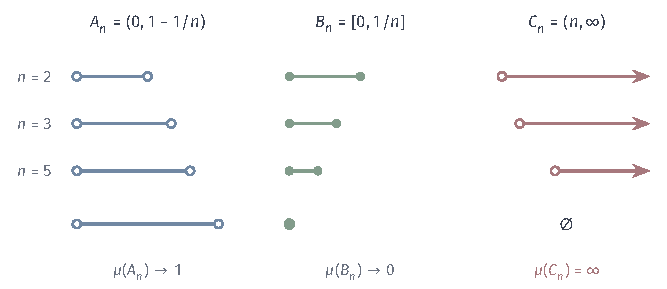
\includegraphics[width=112mm]{figures/01-mathematical-preliminaries-upper/01-mathematical-language-combinatorics-analysis-optimization/tikz/comprehension-additions/nested-set-limits.pdf}
  \caption{实轴上的三列嵌套集合，依次画$n=2,3,5$及最终的并集或交集，均使用勒贝格测度。左列$A_n$递增，并集为$(0,1)$；中列$B_n$递减，交集为$\{0\}$；右列$C_n=(n,\infty)$递减，交集为空，而每一项的测度仍为无穷。空心、实心端点分别表示不包含、包含；各列仅在本列内共用坐标尺度。}
  \label{fig:vol1-add-nested-set-limits}
\end{figure}
\FloatBarrier

\subsubsection{零测集与完备性}
\label{sec:comb-null-sets-and-completion}

集合差的测度可以描述遗漏或多出的总量。当这份总量恰为零时，函数仍可能在其中某些点取不同值，某个性质也可能在那里失效。
我们需要分别说明什么是零测范围、怎样表达范围内允许有例外，以及这些例外的任意子集是否都在可测范围内。
前两个问题引出零测集和几乎处处，最后一个问题引出完备性与完备化。

\paragraph{零测集}

测度为零不等于没有元素：勒贝格长度给单点赋值$0$，点本身却仍然存在。
为了用测量值而非点数描述这种范围，先给它一个名称。
\begin{definition}[零测集]
\label{def:analysis-null-set-almost-everywhere}
在测度空间$(X,\mathcal A,\mu)$中，若$N\in\mathcal A$且$\mu(N)=0$，称$N$为\term{零测集}（null set）。
\end{definition}
单点与所有可数点集在勒贝格测度下都是零测集，因为可数次可加性或次可加性使这些单点的总量仍为零。
在计数测度下，单点的测度却是$1$，唯一的零测集是空集。
因此说一个集合“零测”时，必须同时明确采用什么测度。

\paragraph{几乎处处}

比较两个函数时，除了判断它们是否逐点相等，还可以考察它们不同的位置是否都落在一个零测集中。
下面用同样的方式描述一般性质的例外范围，同时保留所用测度的信息。
\begin{definition}[几乎处处]
若存在可测零测集$N$，使某性质对每个$x\in X\setminus N$成立，称该性质$\mu$-\term{几乎处处}（almost everywhere，简写为a.e.）成立。
\end{definition}
例如$f(0)=1$、$f(x)=0$（$x\neq0$）与恒零函数在勒贝格测度下几乎处处相等，尽管它们在$0$处并不相等。
更进一步，$f=\mathbb I_{Q_0}$在$[0,1]$上也几乎处处等于零，因为例外都在有理点集$Q_0$内。
例外可以在每一小段中出现，所以“几乎处处”不表示只遗漏有限个点，也不表示每个位置附近都没有例外。
按前面有理与无理点的分布，这个指示函数处处不连续，而恒零函数处处连续；几乎处处相等也不会自动保留连续性或某个指定点的取值。
后面讨论积分和函数空间时，会明确哪些结论只依赖零测范围之外的取值。

若一列性质分别在零测集$N_1,N_2,\ldots$之外成立，那么它们在$\bigcup_nN_n$之外同时成立；这个并仍零测。
这使可数多项几乎处处结论能够使用共同的例外范围，但不能直接推广到不可数多项结论。
例如在$[0,1]$上，对每个$t\in[0,1]$，性质$x\neq t$都在勒贝格测度下几乎处处成立；若要求它对所有$t$同时成立，却没有任何$x\in[0,1]$满足。

定义只要求实际例外集包含在某个可测零测集$N$中，没有预先要求例外集自身可测。
这样写是因为一般测度空间可能尚未纳入$N$的全部子集；下面的完备性正要处理这个问题。
计数测度下则没有非空零测例外，几乎处处成立就是处处成立。

\paragraph{Cantor集}
\label{sec:analysis-cantor-set}

可数集是熟悉的勒贝格零测集，但零测是否意味着最多只有可数多个点，还需另行检验。
下面的Cantor集说明，点的数量和长度为零是两种不同的信息。

由$[0,1]$反复删去每段的中间三分之一，得到的\term{Cantor集}（Cantor set）$C$是各层保留集合的交。
第$n$层由$2^n$个长$3^{-n}$的闭区间组成，因此$C$是Borel集合，并满足$m(C)\leq(2/3)^n$对所有$n$成立，故$m(C)=0$。

每条零一序列都可以改写为只用数字$0,2$的三进制数，所得点在$C$中。
两个序列首个不同位的差为$2\cdot3^{-k}$，其后位数的总差至多$3^{-k}$，因此给出不同点。
零一序列不可数：假定列出全部序列，把第$n$条序列的第$n$位取反就得到遗漏的一条。
所以$C$是不可数零测集。零测例外能够包含不可数多个点，几乎处处的表述因此不能用“除去可数多个点”替代。


图~\ref{fig:analysis-process-cantor-deletion}画出上述删除过程：每一步仍有正长度，但这些长度可共同压到任意小，交集却仍保留点。
\begin{figure}[!htbp]
 \centering
 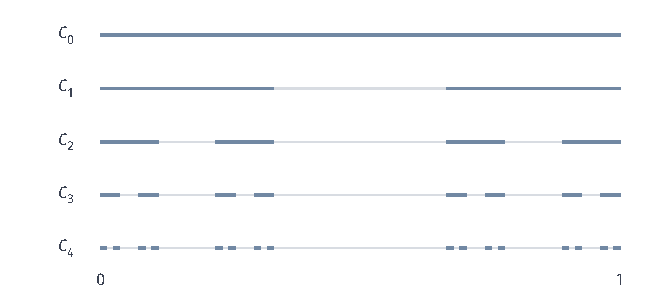
\includegraphics[width=112mm]{figures/01-mathematical-preliminaries-upper/01-mathematical-language-combinatorics-analysis-optimization/tikz/chapter3-concept-processes/cantor-deletion.pdf}
 \caption{蓝线表示$C_0,\ldots,C_4$，每一步从上一行各闭区间中删去中间开三分之一。$C_n$由$2^n$个长度$3^{-n}$的闭区间组成，总长度为$(2/3)^n$；交集$C$的测度因此为零，但始终包含$0,1$。任何有限一行仍有正测度，不能把有限阶段当成最终零测集。}
 \label{fig:analysis-process-cantor-deletion}
\end{figure}

\paragraph{完备性}

设$N$可测且$\mu(N)=0$。若其子集$D\subseteq N$也可测，单调性立即给出$\mu(D)=0$；问题在于$D$未必属于原来的$\mathcal A$。
下面把“所有这种子集都已纳入允许范围”作为一个单独要求。
\begin{definition}[完备测度空间]
\label{def:analysis-complete-measure-space}
若测度空间$(X,\mathcal A,\mu)$中每个零测集$N$的任意子集$D\subseteq N$都属于$\mathcal A$，称该测度空间完备。此时单调性给出$\mu(D)=0$。
\end{definition}
这里的完备性解决零测子集的可测资格，与度量空间中“柯西列是否有域内极限”的完备性是两种不同要求。

例如$X=\{a,b,c\}$、$\mathcal A=\{\varnothing,\{a,b\},\{c\},X\}$，给$\{a,b\}$测度$0$、$\{c\}$测度$1$。
按两块的不交加法确定其他值，就得到一个测度；但$\{a\}\subseteq\{a,b\}$且$\{a\}\notin\mathcal A$，所以它不完备。
在这个空间中，“$x\neq a$”仍几乎处处成立，因为例外被可测零测集$\{a,b\}$包住；此时却不能写$\mu(\{a\})=0$，因为$\mu$尚未在$\{a\}$上定义。
完备空间会消除这种资格上的缺口：被可测零测集包住的例外集自身也可测且为零测。

\paragraph{完备化}

若测度空间不完备，我们希望加入缺少的零测子集，同时保留原来各集合的测量值。
只把零测子集逐个加入还不够，新的允许范围还必须是$\sigma$代数，所以也要允许它们与原可测集组合。

具体把新集合写成“原可测部分$A$加上零测范围内的一部分$D$”，并让$D$不增加总量。
由此定义下面的扩展，随后检查赋值、封闭性和可加性确实成立。
\begin{definition}[测度空间的完备化]
在测度空间$(X,\mathcal A,\mu)$上，令
\[
 \begin{aligned}
 \overline{\mathcal A}&=\left\{A\cup D:
 \begin{array}{l}A,N\in\mathcal A,\quad\mu(N)=0,\\D\subseteq N\end{array}\right\},\\
 \bar\mu(A\cup D)&=\mu(A).
 \end{aligned}
\]
所得$(X,\overline{\mathcal A},\bar\mu)$称为原测度空间的\term{完备化}（completion）。
\end{definition}
取$D=\varnothing$便保留所有原可测集及其测度，取$A=\varnothing$便纳入所有原零测集的子集。
在三点例子中，这会加入$\{a\},\{b\}$及它们与$\{c\}$的并，得到全部子集；原来两块的测度仍为$0$与$1$。

首先要检查同一新集合的不同表示不会给出不同数值。
若$A\cup D=A'\cup D'$，其中$D\subseteq N$、$D'\subseteq N'$，则可测差集$A\setminus A'\subseteq N'$、$A'\setminus A\subseteq N$都为零测。
把$A,A'$各拆成公共部分与差集，有限可加性给出$\mu(A)=\mu(A\cap A')=\mu(A')$，即赋值与表示无关；这里没有使用可能无意义的无穷值相减。

其次检查新的范围对所需运算封闭。全集已在原范围内；取补时，
\[
 X\setminus(A\cup D)=[X\setminus(A\cup N)]\cup[N\setminus(A\cup D)],
\]
第一项原本可测，第二项是原可测零测集$N$的子集，仍是允许的新表示。
可数并也保持这种形式：$\bigcup_j(A_j\cup D_j)=(\bigcup_jA_j)\cup(\bigcup_jD_j)$，
而$\bigcup_jD_j\subseteq\bigcup_jN_j$，右侧是原可测零测集。
所以$\overline{\mathcal A}$确实是$\sigma$代数。

再检查测量规则。若$A_j\cup D_j$两两不交，它们的可测部分$A_j$也两两不交，故
\[
 \bar\mu\left(\bigcup_j(A_j\cup D_j)\right)
 =\mu\left(\bigcup_jA_j\right)
 =\sum_j\mu(A_j)=\sum_j\bar\mu(A_j\cup D_j).
\]
空集的值也仍为零，因此$\bar\mu$是测度。
若新可测集$A\cup D$的测度为零，则$\mu(A)=0$，整个集合包含在原可测零测集$A\cup N$中。
它的任意子集都已按新规则纳入，故扩展后的空间完备。

这些加入也是必要的：任何保留原测度的完备扩展，都必须包含原零测集的所有子集及它们与原可测集的并。
所以完备化给出的正是满足这一要求所需的最小可测范围，并未任意改变已有测量规则。
引理~\ref{lem:analysis-zero-outer-measure-measurable}已经保证勒贝格零测集的全部子集可测且仍零测，所以勒贝格测度本身已经完备。
接下来将用集合逼近说明：从Borel长度出发进行完备化，恰好得到完整的勒贝格可测范围。

\subsubsection{集合的逼近}

集合列的连续性回答了“给定一列嵌套集合，最终并或交有多大”；现在要反过来问：给定一个可测集，能否为它找到容易描述的近似集合？
开集、闭集和有限区间并可以用区间或有限组合描述，若能控制它们与原集合之间多出、漏掉部分的测度，就能把一般集合的问题转为简单集合的计算。

下面回到实轴上的勒贝格测度，使用它的开区间覆盖构造与实轴拓扑。
这些内外逼近不是任意测度空间自动具有的性质；一般的$(X,\mathcal A,\mu)$甚至还没有指定开集、闭集的含义。

\paragraph{内外正则性}

从外面逼近要求开集$O$包含全部$E$，只允许多出少量测度；从里面逼近要求有界闭集$K$完全落在$E$内，只允许漏掉少量测度。
下面把“少量”写成任意正误差，并保留控制余量所需的有限测度条件。
\begin{theorem}[有限测度集合的内外逼近]
设$E\in\mathcal L(\mathbb R)$且$m(E)<\infty$。对任意$\varepsilon>0$，存在开集$O$和有界闭集$K$满足
\begin{equation}
 K\subseteq E\subseteq O,\qquad
 m(O\setminus E)<\varepsilon,\qquad m(E\setminus K)<\varepsilon.
 \label{eq:comb-lebesgue-set-approximation}
\end{equation}
\end{theorem}
这就是本处使用的勒贝格测度正则性。这里控制的是多出、漏掉的测度，不要求集合边界在距离意义下彼此接近。
例如$E=[0,1]$可取$K=[0,1]$、$O=(-\varepsilon/3,1+\varepsilon/3)$，外面多出的长度为$2\varepsilon/3$，里面没有遗漏。

\begin{proof}
先作外逼近。由$m(E)=m^*(E)$的覆盖定义，选择总长度小于$m(E)+\varepsilon$的开区间覆盖，令$O$为这些区间的并。
它是可测开集，且$E\subseteq O$、$m(O)\leq\sum_j\ell(I_j)<m(E)+\varepsilon<\infty$。
把$O$分成不交的$E$与$O\setminus E$，可得$m(O\setminus E)=m(O)-m(E)<\varepsilon$。

内逼近分两步处理：先控制远处尾部，再在有限区间内对补集作外逼近。
因为$E\cap[-M,M]\uparrow E$，下连续性及$m(E)<\infty$保证可以取正整数$M$使
$m(E\setminus[-M,M])<\varepsilon/2$。
令$F=[-M,M]\setminus E$，它可测且测度有限。
应用刚才的外逼近，选开集$U\supseteq F$使$m(U\setminus F)<\varepsilon/2$，并令
\[
 K=[-M,M]\setminus U.
\]
$K$是有界闭集；由于已经去掉整个$F$，它包含于$E$。
遗漏部分分为区间外的尾部与区间内落入$U$的部分，因而
\[
 \begin{aligned}
 m(E\setminus K)
 &\leq m(E\setminus[-M,M])+m(U\setminus F)\\
 &<\varepsilon/2+\varepsilon/2=\varepsilon.
 \end{aligned}
\]
这就同时给出内外两种估计。
\end{proof}
有限性在证明中用于控制远处尾部并允许相减。若$E=\mathbb R$，任取有界闭集$K$，都有$m(E\setminus K)=\infty$，不可能达到上述任意小遗漏要求。
所以不能将本定理中“有界闭集的内逼近”直接照搬到无限测度集合；处理一般集合时，可以先限制在$[-M,M]$中作局部逼近。

图~\ref{fig:measure-inner-outer}将多出与漏掉的范围放在同一坐标尺度下。孤立点虽须包含于外覆盖，却可能在内逼近中被遗漏而不增加测度误差。

\begin{figure*}[htbp]
 \centering
 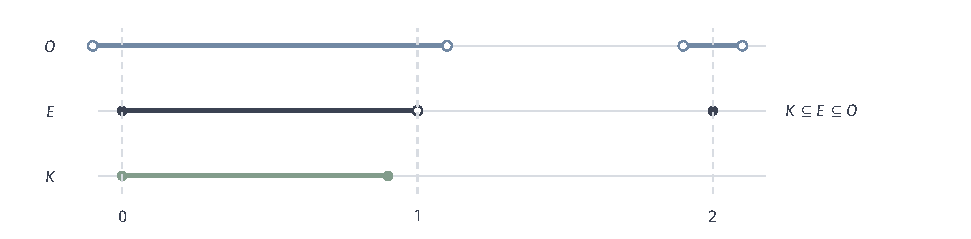
\includegraphics[width=169mm]{figures/01-mathematical-preliminaries-upper/01-mathematical-language-combinatorics-analysis-optimization/tikz/measure-inner-outer/figure.pdf}
 \caption{内外逼近控制的是集合差的测度。取$E=[0,1)\cup\{2\}$、有界闭集$K=[0,0.9]$及开集$O=(-0.1,1.1)\cup(1.9,2.1)$，有$K\subseteq E\subseteq O$。外面多出的长度$m(O\setminus E)=0.4$，里面遗漏的长度$m(E\setminus K)=0.1$；遗漏孤立点$2$不增加长度。空心端点不包含，实心端点包含。该图给出一次具体逼近，任意小误差由正文定理保证。}
 \label{fig:measure-inner-outer}
\end{figure*}


\paragraph{有限区间并}

开集和有界闭集仍可能包含无限结构。为了得到真正有限的计算对象，还希望用有限个区间的并逼近$E$。
这里改为同时控制多出和漏掉的总量，不要求这个有限区间并一定包含$E$或包含于$E$。

若$E=\varnothing$，直接取空集作为有限区间并即可。以下设$E$非空且可测、$m(E)<\infty$，给定$\varepsilon>0$，先取开集$O\supseteq E$使$m(O\setminus E)<\varepsilon/2$。
此时$m(O)<\infty$。把$O$写成其中有理端点开区间的可数并，令$O_N$为前$N$个区间之并，则$O_N\uparrow O$。
由下连续性，$m(O_N)\to m(O)$；总量有限，便有$m(O\setminus O_N)\to0$。
可选$N$使$m(O\setminus O_N)<\varepsilon/2$。
若所用区间只有有限个，可以重复已有区间补成一列。

记所得有限区间并为$B=O_N$。两方向的误差分别满足
$E\setminus B\subseteq O\setminus O_N$、$B\setminus E\subseteq O\setminus E$。
将它们合在一起，定义对称差$E\triangle B=(E\setminus B)\cup(B\setminus E)$，便有
\[
 m(E\triangle B)=m(E\setminus B)+m(B\setminus E)<\varepsilon.
\]
这称为在测度意义下逼近：误差是两集合不同之处的测度，而不是点的位置误差。
它与Jordan内外夹逼的要求不同。例如$E=Q_0$时，取$B=\varnothing$就有$m(E\triangle B)=0$，尽管两个集合并不相等。
这不构成Jordan外部逼近，因为空集并没有覆盖$Q_0$；所以这里的有限区间并逼近不与前面Jordan外容量为$1$的结论矛盾。
集合的这种逼近也不自动保证任意函数的积分误差很小，后面还需要对函数另加控制条件。

\paragraph{Borel范围的完备化}

完备化规定怎样加入零测子集，内外逼近则能说明一般勒贝格可测集与Borel集合究竟差在哪里。
下面证明每个勒贝格可测集都能写成Borel集合加上Borel零测集的一部分，因此Borel长度的完备化正好得到勒贝格范围。

先设$m(E)<\infty$。对每个$n$选有界闭集$K_n\subseteq E$使$m(E\setminus K_n)<2^{-n}$，令
\[
 F=\bigcup_{n=1}^{\infty}K_n.
\]
$F$是Borel集合且$F\subseteq E$。由于$E\setminus F\subseteq E\setminus K_n$对每个$n$成立，
$m(E\setminus F)\leq2^{-n}$对所有$n$成立，所以$m(E\setminus F)=0$。
这已给出一个内部Borel部分，但完备化的定义还要求把余量放入原范围中的零测集，因此需进一步找一个Borel零测集来包住它。

记$D=E\setminus F$。由外逼近，对每个$n$取开集$O_n\supseteq D$使$m(O_n)<2^{-n}$。
令$N=\bigcap_nO_n$，则$N$是Borel集合、$D\subseteq N$，且$m(N)\leq m(O_n)<2^{-n}$对所有$n$成立，故$m(N)=0$。
于是$E=F\cup D$，其中$F$为Borel集合，$D$包含于Borel零测集$N$，正是完备化允许加入的形式。

若$m(E)$无限，先对每个$E_k=E\cap[-k,k]$作上述构造，写成$E_k=F_k\cup D_k$、$D_k\subseteq N_k$。
取$F=\bigcup_kF_k$、$D=\bigcup_kD_k$、$N=\bigcup_kN_k$，便有$E=F\cup D$、$D\subseteq N$，
其中$F,N$均为Borel集合，$N$由可数次可加性仍为零测。
因此每个勒贝格可测集都进入Borel长度测度的完备化。

反过来，Borel集合已经勒贝格可测，Borel零测集的任意子集又因勒贝格完备性而可测，
所以完备化加入的集合不会超出勒贝格范围。
两个方向合起来证明，实轴上的勒贝格测度空间就是Borel长度测度空间的完备化，已有Borel集合上的长度保持不变。

到此，可数可加性使集合列的测度可以取极限，零测集给出几乎处处的例外语言，完备化补齐这类例外的子集，
内外逼近则把一般可测集联系到开闭集和有限区间并，并解释了Borel范围与勒贝格范围的关系。
下一节建立积分时，将使用这些可测范围、测量值以及控制误差的工具来累计函数取值。

\FloatBarrier
